\section{Analysis and Discussion}

\subsection{Experimental Design}

To comprehensively evaluate the performance of different methods under varying problem scales and constraints, we construct nine distinct scenarios, each defined by a unique combination of total participant number $n \in \{50, 300, 1000\}$ and maximum group size $s_{\max} \in \{15, 30, 50\}$. For each scenario, we generate three randomized instances using different seeds ($\text{seed} \in \{0, 1, 2\}$), resulting in a total of 27 experiments.

In each instance, we synthetically generate two key data matrices:
\begin{itemize}
    \item \textbf{Diversity Matrix} $D \in \mathbb{R}^{n \times n}$: Created using a clustered distribution to simulate affinity-based or subgroup-specific dissimilarities among participants.
    \item \textbf{Engagement Vector} $E \in \mathbb{R}^n$: Generated from a normal distribution to simulate varying levels of individual engagement or willingness to contribute.
\end{itemize}

Each method is evaluated based on its assignment of individuals into groups, subject to group size constraints (no more than $s_{\max}$ per group). The objective is to maximize overall diversity within groups while maintaining balanced engagement across them. The weighting parameters for the objective function are set to $\lambda_1 = 1.0$ and $\lambda_2 = 0.0001$.

The methods compared include:
\begin{itemize}
    \item \textbf{Naive Baseline}: Random modulo-based assignment.
    \item \textbf{Heuristic Composite (Random Improvement iteration)}: An iterative method combining subgradient optimization and local search, with a maximum of 2000 iterations.
    \item \textbf{Integer Programming (IP) with Lagrangian Relaxation}: Solved via Gurobi, using binary variables and a decomposition-based reformulation. The solver runs for up to 600 iterations.
    \item \textbf{Linear Programming (LP) Relaxation with Lagrangian Relaxation}: Similar to IP, but allows fractional group assignment variables in $[0, 1]$, also capped at 600 iterations.
\end{itemize}

For each method and instance, we record the following metrics:
\begin{itemize}
    \item \textbf{Optimality Gap (\%)}: Relative gap to the IP+Lagrangian solution (baseline).
    \item \textbf{Execution Time (s)}: Measured using wall-clock time via \texttt{time.perf\_counter()}.
\end{itemize}

All results are aggregated by scenario and reported as averages across three seeds. The IP+Lagrangian method serves as the reference for computing optimality gaps.


\subsection{Motivation for Lagrangian Approach}

Solving the full integer program (IP) to optimality is computationally intensive and becomes intractable for large-scale group deliberation scenarios, especially when the number of participants and grouping constraints increase. In our preliminary tests, even with a powerful solver like Gurobi, solving the exact IP model required hundreds of seconds per instance. To alleviate this, we introduce a Lagrangian-based decomposition approach that retains modeling fidelity while significantly reducing computation time.

Instead of relying on brute-force search or complete enumeration, we reformulate the group assignment problem using Lagrangian relaxation to decouple constraints, enabling more efficient optimization. In practice, we set the maximum number of iterations to \textbf{2000} for the heuristic method, and \textbf{600} for both the IP with Lagrangian relaxation and LP relaxation, ensuring a fair and controlled comparison across methods.

\subsection{Baseline Comparisons}

To evaluate the effectiveness of the proposed Lagrangian Decomposition (LD) method for the group assignment problem, we compare it against the following baselines:

\begin{itemize}
    \item \textbf{Naive Baseline}: Random assignment without any optimization.
    \item \textbf{Heuristic Composite}: A custom-designed heuristic using subgradient methods and local search to iteratively improve solutions as mentioned above.
    \item \textbf{Integer Programming (IP) with Lagrangian Relaxation}: Solved using Gurobi with binary decision variables and Lagrangian reformulation.
    \item \textbf{Linear Programming (LP) Relaxation with Lagrangian Relaxation}: Similar to IP but relaxes binary variables to continuous values in $[0, 1]$.
\end{itemize}

The first two approaches are solver-free and scalable, while the latter two serve as performance upper bounds using commercial optimization software.

\subsection{Performance Metrics}

We use the following metrics to evaluate each method:

\begin{itemize}
    \item \textbf{Optimality Gap (\%)}: Measures how far a method's solution is from the best-known IP value. As this is a maximization problem, the gap is defined as:
    \[
    \text{Gap} = \frac{\text{Optimal Value} - \text{Method Value}}{|\text{Optimal Value}|} \times 100
    \]
    A smaller gap indicates a better solution.
    
    \item \textbf{Standard Deviation (Std)}: Captures the variation in results across repeated trials and reflects robustness.
    
    \item \textbf{Execution Time (seconds)}: Measures the average runtime of each method, important for practical deployment and scalability.
\end{itemize}

All experiments were conducted on the same hardware platform (Apple M-series CPU), and each setting was repeated three times to compute averages and deviations.

\subsection{Optimality Gap}

\textbf{Average Optimality Gap by Scenario} illustrates the average optimality gaps across nine different scenarios, defined by combinations of $(n, s_{\max})$. The IP Lagrangian solution serves as the benchmark baseline (gap = 0\%). 

Among the three heuristics, the \textbf{Random Improvement Iteration Heuristic} consistently outperformed the Naive heuristic. For instance, in the largest instance $(n=1000, s_{\max}=15)$, the CHSF gap was approximately 75.0\%, compared to 887.1\% for the Naive heuristic—a reduction of over 91\%. Even in the smallest case $(n=50, s_{\max}=15)$, Random Improvement Iteration yielded a gap of 16.2\%, still substantially lower than the Naive heuristic’s 140.2\%.

The LP Relaxation method achieved near-zero gap in most scenarios (0\% except 0.4\% in the largest instance), affirming its tight bound but at the cost of high computation time, as discussed below.

\begin{figure}[H]
    \centering
    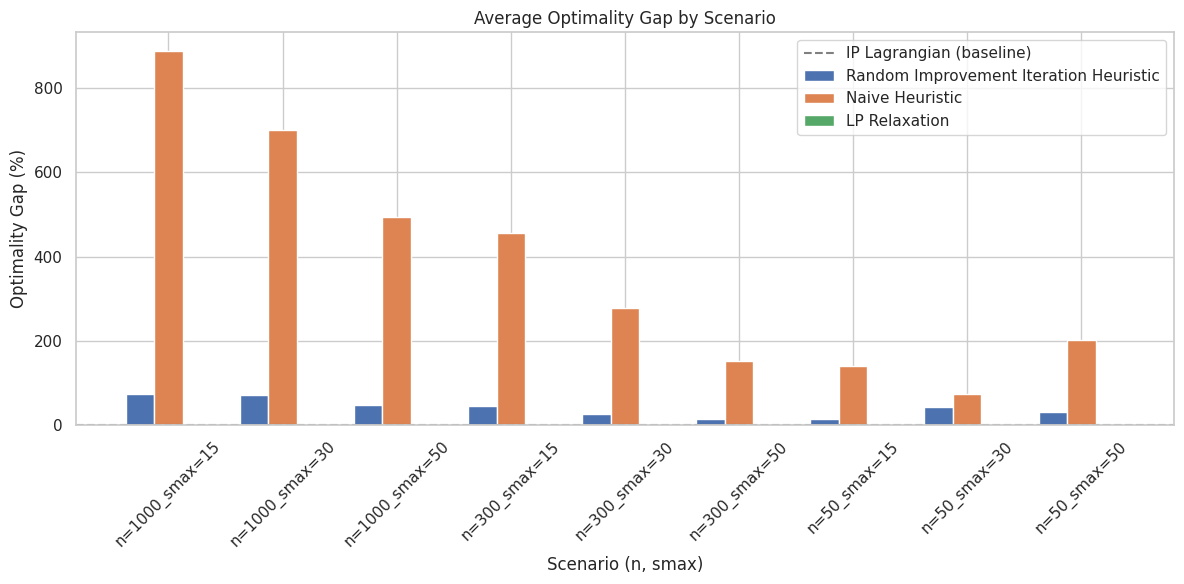
\includegraphics[width=0.8\textwidth]{assets/gap.png}
    \caption{Average Optimality Gap by Scenario}
    \label{fig:your-label}
\end{figure}

\subsection{Computation Time}

\textbf{Figure 2} presents the average computation time on a logarithmic scale. While the Naive heuristic completed in under 0.01 seconds for all scenarios (e.g., 0.007s in $(n=1000, s_{\max}=15)$), Random Improvement Iteration required more time due to its iterative improvement steps—e.g., 1.35s in the same instance. Nevertheless, this is still orders of magnitude faster than LP Relaxation, which took over 413 seconds.

Interestingly, Random Improvement Iteration provided a strong balance between solution quality and computational efficiency. Across all settings, it achieved substantial gap reduction compared to the Naive approach while keeping runtime within practical limits (all under 1.4 seconds). 

\begin{figure}[H]
    \centering
    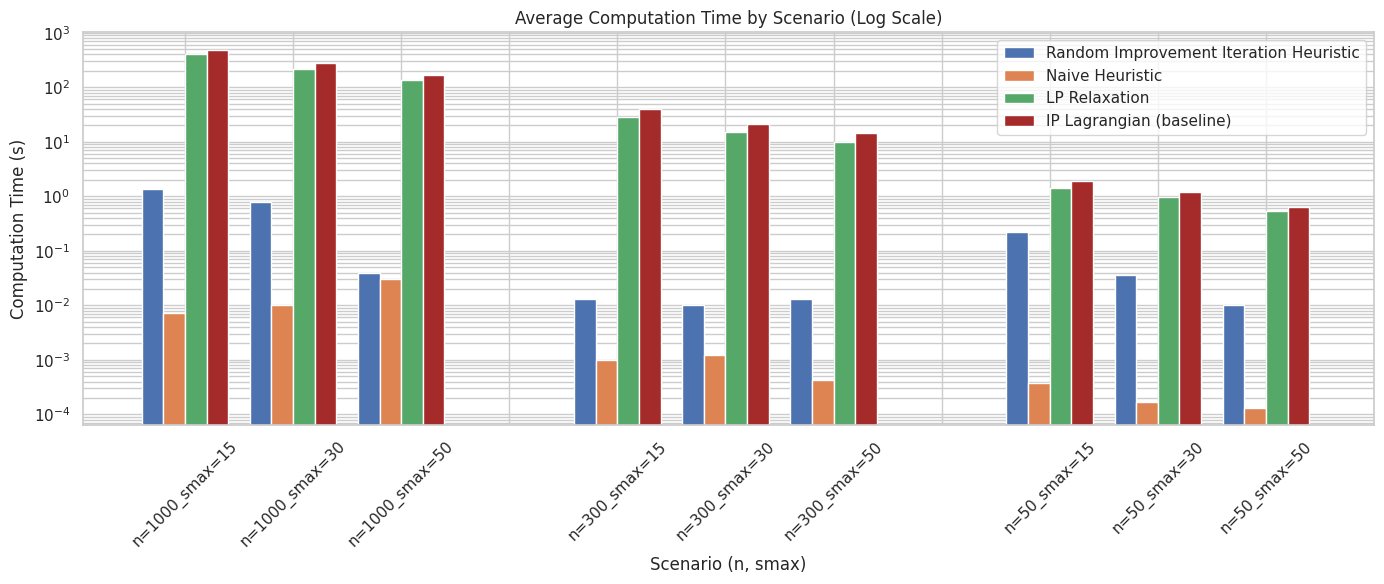
\includegraphics[width=0.8\textwidth]{assets/time.png}
    \caption{Average Computation Time by Scenario (Log Scale)}
    \label{fig:your-label}
\end{figure}

\subsection{Summary}

In summary, the Random Improvement Iteration heuristic demonstrates clear advantages over the Naive baseline in both optimality and scalability. It also provides a viable alternative to LP Relaxation when computational cost is a limiting factor, especially for large-scale instances.

In conclusion, the proposed \textbf{Lagrangian-based heuristic provides a compelling trade-off between solution quality and runtime}. It is especially suitable for large-scale, real-time, or resource-constrained scenarios. Furthermore, the modular structure of the heuristic framework makes it extendable to more general group assignment settings, including multi-objective, multi-stage, or incomplete-information environments.
